\documentclass[twoside]{article}
\usepackage{lmodern}
\usepackage{listings}
\usepackage{amsmath}
\usepackage{amssymb}
\usepackage{graphicx}
\title{Artificial Intelligence}
\date{}
\author{}
\begin{document}
\maketitle
\section{What is an AI?}
There are various definitions of an AI, ranging from thinking humanly and
rationally to acting humanly and rationally. The \emph{turing test}, is test
in which a human interrogator interacts with a machine, sending it messages
back and forth, and a machine passes if it fools the human into thinking that
the messages are being sent to them by a human. For this a computer needs:
\textbf{natural language processing, knowledge representation, automated
reasoning and machine learning}. To pass the \emph{total turing test} a computer
would additionally need \textbf{computer vision and robotics.}
\subsection{Intelligent Agents}
An \textbf{agent} is just something that acts and a \textbf{rational agent} is
one that acts so as to achieve the best outcome or, when there is uncertainty,
the best expected outcome. \textbf{Percept} means the agent's perceptual inputs
at any given time, and a \textbf{percept sequence} is the complete history of
everything the agent has ever perceived. The \textbf{agent function} is an
abstract mathematical description that maps a given percept to an action; an
\textbf{agent program} is a concrete implementation of the agent function, running within some
physical system. \emph{It is better to design a performance measure according
to what one wants in an environment, then how one wants an agent to behave.}
\\ \\
The proper definition of a rational agent is \emph{for each possible percept
sequence, a rational agent should select an action that is expected to
maximize its performance measure, given the evidence provided by the percept
sequence and whatever built-in knowledge the agent has.} An \textbf{omniscient}
agent knows the actual outcomes of its actions.
\subsection{The Nature of Environments}
An environment is defined as \textbf{PEAS}: performance measure, environment,
actuators and sensors. There are different types of environments, namely:
\begin{itemize}
\item \textbf{Observable vs Partially-Observable}: it is observable when the agents'
        sensors have complete access to the environment's state at all times.
\item \textbf{Single agent vs Multi agent}: there could be multiple agents in
        an environment. There is also a question of what must be considered as an
        agent. This gives way to the concept of \textbf{competitive} vs
        \textbf{cooperative} environments.
\item \textbf{Deterministic vs Stochastic}: if the next state can be completely
        determined by the current state and the action executed by the agent,
        then it is deterministic; and stochastic otherwise. An environment
        is \textbf{uncertain} if it is not fully observable or not deterministic.
        Note that a \textbf{non-deterministic} environment is one where each
        action is characterized by its possible outcomes, but no probabilities
        are attached to them.
\item \textbf{Episodic vs Sequential}: in an episodic environment the agent's
        experience is divided into atomic episodes. The next episode doesn't
        depend on the action taken in the previous episode.
\item \textbf{Static vs Dynamic}: if an environment can change when an agent
        is deliberating, then it's dynamic, and is static otherwise. If the
        environment doesn't change when deliberating but the performance score
        does, then we call it \textbf{semi-dynamic.}
\item \textbf{Discrete vs Continuous}: the distinction here applies to the state
        of the environment, the way time is handled and the percepts and actions
        of the agent. For example, chess having a discrete set of states; the
        same doesn't apply for taxi driving.
\item \textbf{Known vs Unknown}: this applies to the agent's state of knowledge
        about the ``laws of physics'' of the environment. Note that it's 
        possible that a known environment is partially observable like solitaire.
        Conversely, an environment can also be unknown and fully observable,
        like in a video game, one can see the state but one doesn't know the
        control until one tries to play.
\end{itemize}
\subsection{The Structure of Agents}
There are four basic types of agent programs:
\begin{itemize}
        \item \textbf{Simple Reflex Agents}: Agents that select the current
        action based on the current precepts and ignoring the rest of the
        precept history. It is also important to note that these types of
        agents are usually implemented in a fully-observable environment.
        \item \textbf{Model-Based Reflex Agents}: The best way to handle a
        partially observable environment is to keep some sort of an internal
        representation of the aspects of the environment not currently
        observable. Therefore, an agent should have some sort of knowledge
        about how the world works and the agents who have said knowledge are
        called model-based agents.
        \item \textbf{Goal-Based Agents}: These types of agents consider how
        close they get to a goal, in addition to having a model of how their
        environment works. These types of agents are also quite flexible as
        they can update their actions on-the-fly depending on their goals and
        the feedback they get from the environment.
        \item \textbf{Utility-Based Agents}: Since the previous model does not
        differentiate between how it gets to its goal, and which state would
        make it more happy, it is not efficient. Therefore a utility function
        is needed to determine just that i.e. it is an internalization of its
        performance measure. The previous model will also fail when there are
        conflicting goals or when there are several goals the agent can aim
        for, none of which can be achieved with certainty; in both cases,
        a utility function can dictate which action to take to maximize
        expected utility.
\end{itemize}
There are different ways an agent can represent the world around it:
\begin{itemize}
        \item \textbf{Atomic}: Each state is of the world is indivisible: it
        has no internal structure.
        \item \textbf{Factored}: Each state is split up into a fixed set of
        variables and attributes, each of which can have a value. Uncertainty
        can also be represented in this representation.
        \item \textbf{Structured}: This type of representation has objects and
        their relationships with each other.
\end{itemize}

\section{Problem Solving by Searching}

\textbf{Goal formulation}, based on the current situation and the agent's
performance measure, is the first step in problem solving. \textbf{Problem 
formulation} is the process of deciding what actions and states to consider,
given a goal. In general, \emph{an agent with several immediate options of 
unknown value can decide what to do by first examining future actions that 
eventually lead to states of known value.} The process of looking for a 
sequence of actions that reaches the goal is called \textbf{search}. A search
algorithm takes a problem as input and returns a \textbf{solution} in the 
form of an action sequence. Once a solution is found, the actions it recommends
can be carried out. This is called the \textbf{execution} phase. Note that while
the agent is executing, it \emph{ignores its percepts} when choosing its actions
because it knows in advance what they will be.\\

Together, the \textbf{initial state, actions and transition model} implicitly
define the \textbf{state space} of the problem - the set of all states
reachable from the initial state by any sequence of actions. A \textbf{solution}
to a problem is an action sequence that leads from the initial state to a goal
state. Solution quality is measured by the path cost function, and an \textbf{
optimal solution} has the lowest path cost among all solutions. The process 
of removing detail from a representation is called \textbf{abstraction}.\\

It is quite important to distinguish between a node and a state: a node is a 
bookkeeping data structure used to represent the search tree. A state 
corresponds to a configuration of the world. Furthermore, two different nodes
can contain the same world state if that state is generated via two different
search paths. We can evaluate the performance of an algorithm in four ways:
\begin{itemize}
    \item \textbf{Completeness}: Is the algorithms guaranteed to find a solution
    if there is one?
    \item \textbf{Optimality}: Does the strategy find the optimal solution?
    \item \textbf{Time complexity}: How long does it take to find a solution?
    \item \textbf{Space complexity}: How much memory is needed to perform the
    search?
\end{itemize}
In AI, the graph is often represented implicitly by the initial state, actions
and transition model and is frequently infinite. Complexity is expressed in
terms of three quantities: \emph{b}, the \textbf{branching factor} or maximum
number of successors of any node; \emph{d}, the \textbf{depth} of the shallowest
goal node; and \emph{m}, the maximum length of any path in the state space.

\subsection{Uninformed Search Strategies}
\subsubsection{Breadth-First Search}
This is a simple strategy in which all the nodes are expanded at a given depth
in the search tree before any nodes at the next level are expanded. The 
algorithm is given in figure \ref{fig:bfs}.

\begin{figure}
  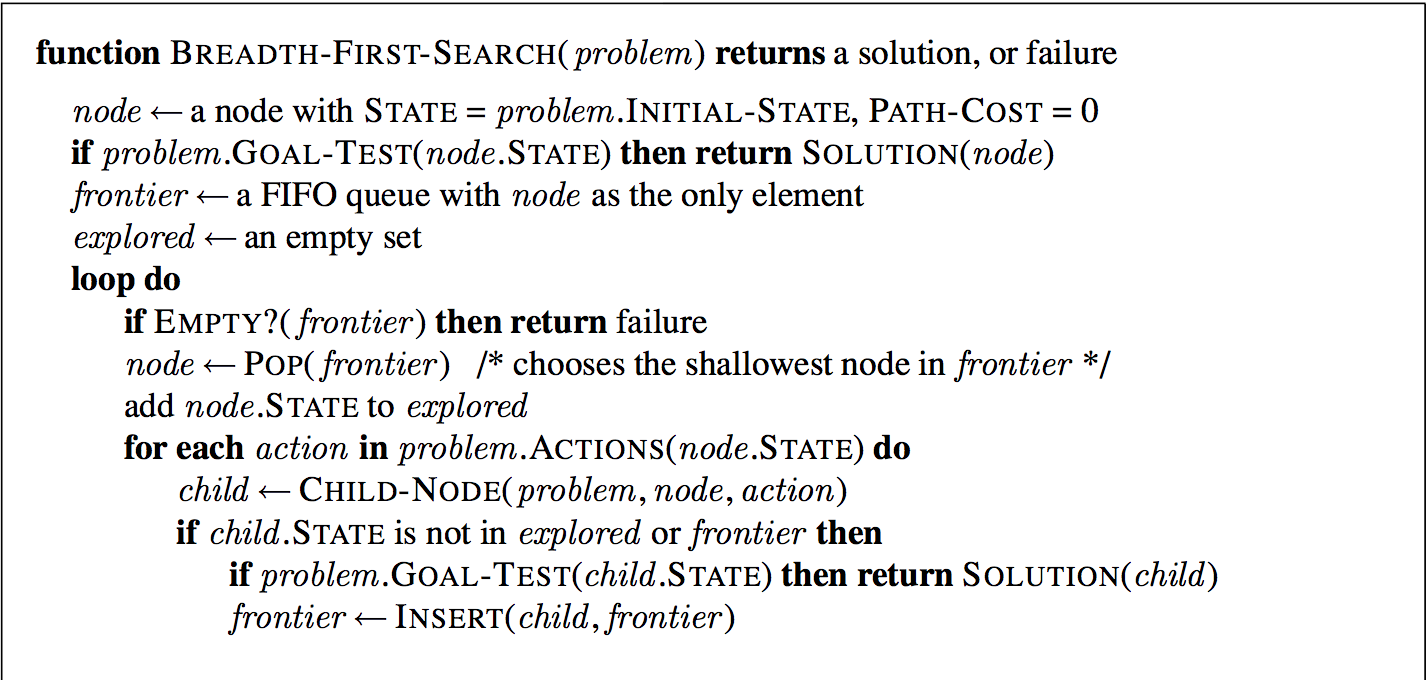
\includegraphics[width=\linewidth]{bfs.png}
  \caption{Breadth-First Search.}
  \label{fig:bfs}
\end{figure}
BFS is \emph{complete} - if the shallowest goal node is at some finite depth
BFS will eventually find it after generating all the shallower nodes. Note
that the \emph{shallowest} is not always the \emph{optimal} one. BFS is only 
optimal if the path cost is a non-decreasing function of the depth of the node.
The time complexity of BFS is:
\begin{equation}
    b + b^2 + b^3 + ... + b^d = O(b^d)
\end{equation}
For the space complexity there will be \(O(b^{d-1})\) nodes in the explored set 
and \(O(b^{d})\) nodes in the frontier, giving space complexity as \(O(b^{d})\).
\emph{Memory requirements are a bigger problem for BFS than execution time and
time is still a major factor. Exponential-complexity search problems cannot
be solved by uninformed methods for any but the smallest instances.}

\subsubsection{Uniform-Cost Search}
This is similar to BFS, but it expands the node with the lowest path cost, the
goal test is applied to a node \emph{not when it's generated, but when it's
chosen for expansion} and a test is added in case a better path is found to a
node currently on the frontier. The algorithm is given in figure \ref{fig:ucs}.
First, we note that whenever this algorithm selects a node for expansion, the 
optimal path to that node is found and second, paths never get shorter as
nodes are added. Thus, \emph{uniform-cost search expands nodes in order of 
their optimal path cost.} This search is complete given that the cost of every
step exceeds some small positive constant \(\epsilon\). The space and time
complexity is \(O(b^{1+\lfloor C^*/\epsilon \rfloor})\), where \(C^*\) is the
cost of the optimal solution.
\begin{figure}
  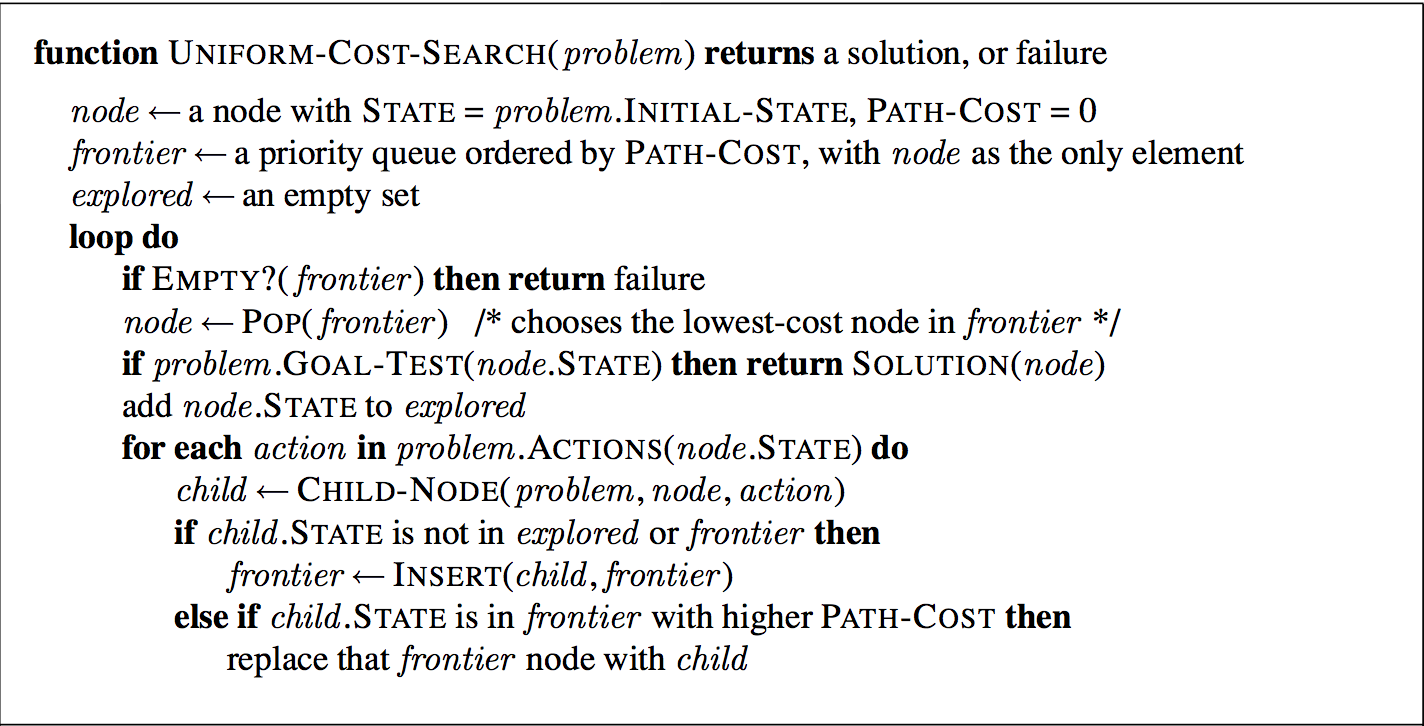
\includegraphics[width=\linewidth]{uniform.png}
  \caption{Uniform-Cost Search.}
  \label{fig:ucs}
\end{figure}
\subsubsection{Depth-First Search}
Depth-First Search always expands upon the deepest node in the frontier, this
is accomplished using a LIFO queue. The graph-search version of the algorithm
is complete in finite spaces but the tree-search version could potentially
fall into a infinite loop. Although, it must be noted that both versions fail
if there is an infinite state space, with an infinite non-goal path e.g.
Knuth's 4 problem. Both versions are also not optimal. The time complexity of
DFS is \(O(b^m)\) and space complexity is \(O(bm)\).
\begin{figure}
  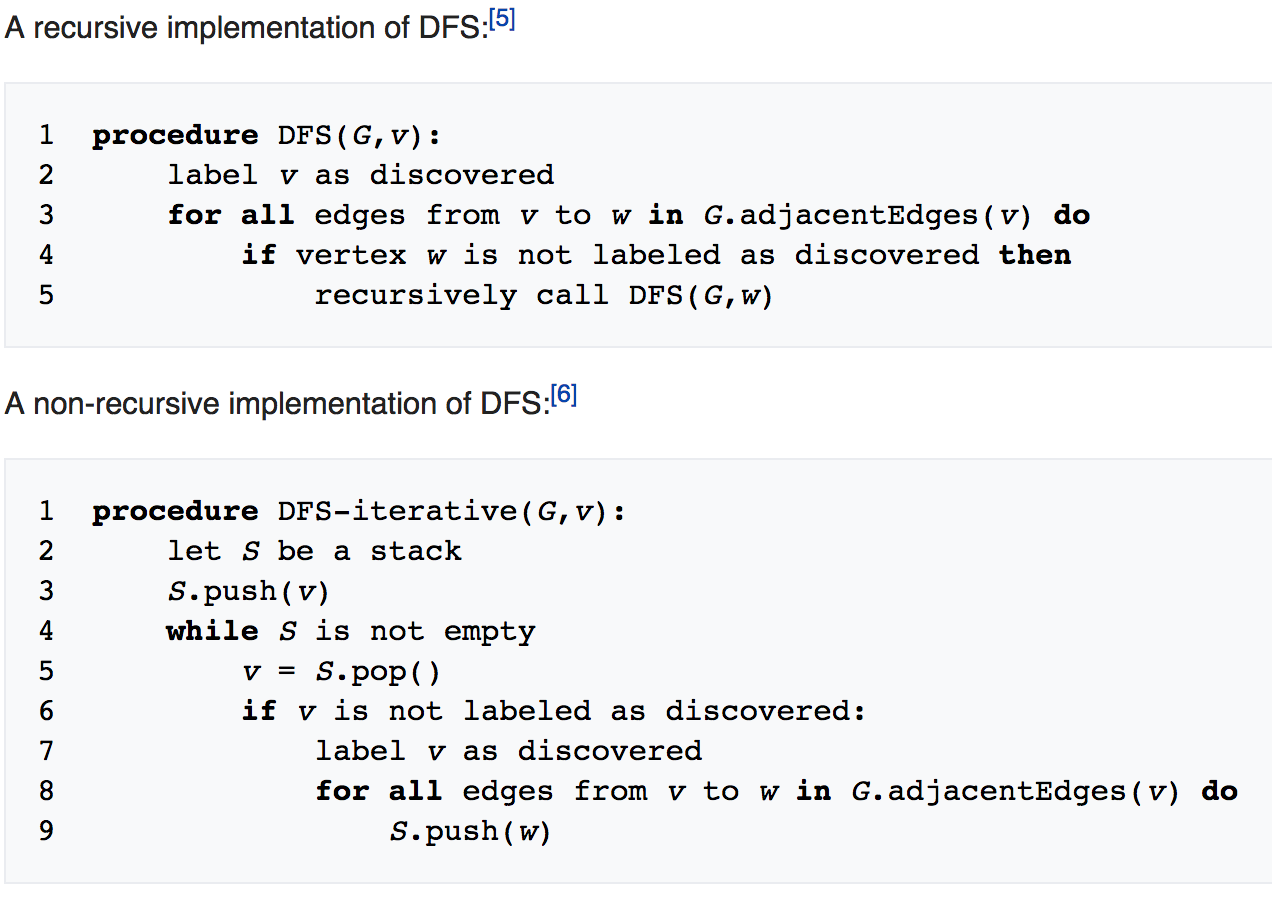
\includegraphics[width=\linewidth]{dfs.png}
  \caption{Depth-First Search.}
  \label{fig:dfs}
\end{figure}
\subsubsection{Depth-Limited Search}
The problem of DFS failing in infinite spaces can be solved if we apply a
limit \(\ell\) to the depth we expand up till. Although, it introduces 
incompleteness if we choose \(\ell < d\) and non-optimality if \(\ell > d \). Its 
time complexity is \(O(b^\ell)\) and its space complexity is \(O(b\ell)\). Its 
pseudocode is shown in figure \ref{fig:dls}.
\begin{figure}
  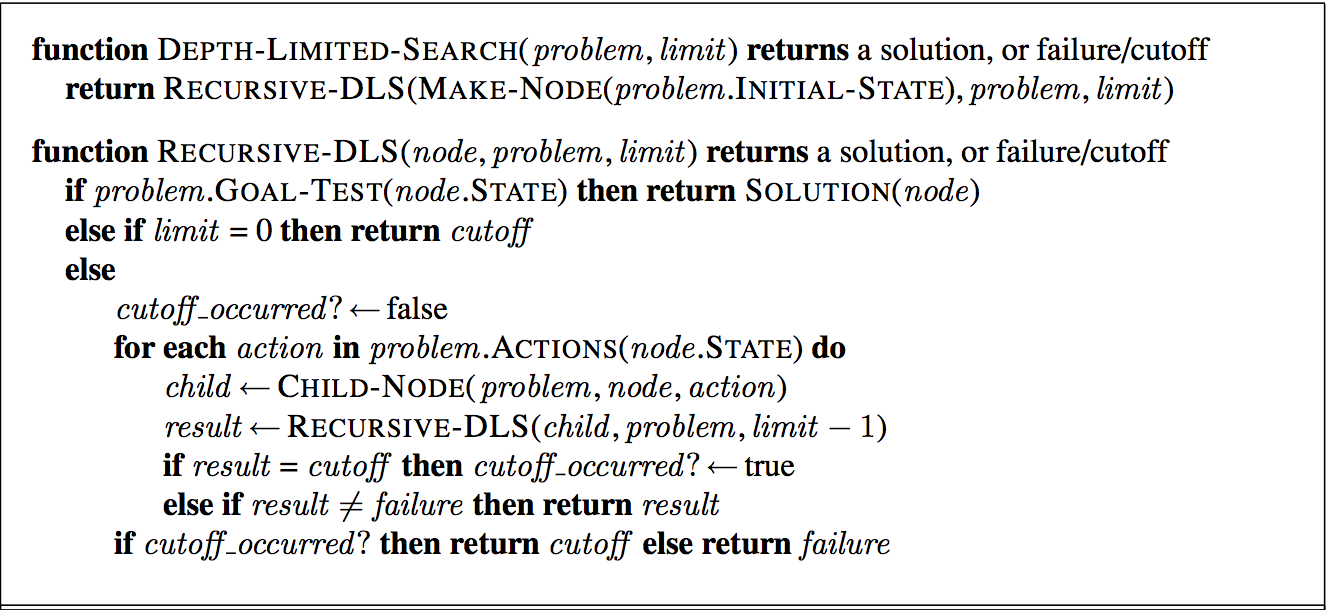
\includegraphics[width=\linewidth]{dls.png}
  \caption{Depth-Limited Search.}
  \label{fig:dls}
\end{figure}
\subsubsection{Iterative Deepening Search}
The algorithm of IDS is shown in figure \ref{fig:ids}. Its space complexity
is \(O(bd)\). Like BFS, IDS is complete if the branching factor is finite and
it is optimal when the path cost is a non-decreasing function of the depth.
The time complexity is:
\begin{equation}
    (d)b + (d - 1)b^2 + ... + (d - d + 1)b^d = O(b^d)
\end{equation}
\emph{In general, IDS is preferred if the search space is large and the depth
of the solution is not known.}
\begin{figure}
  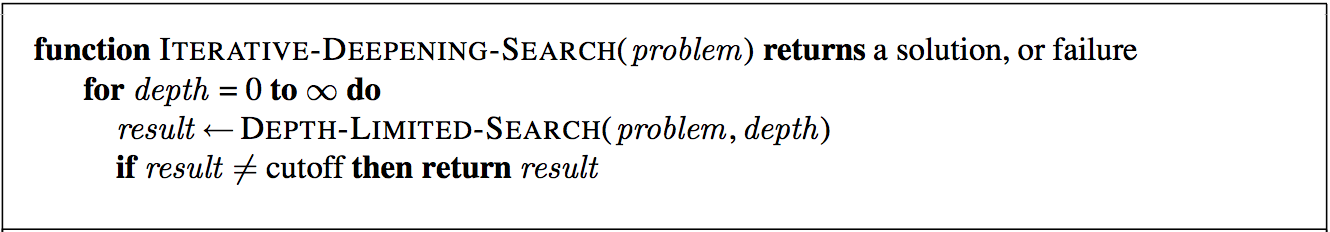
\includegraphics[width=\linewidth]{ids.png}
  \caption{Iterative Deepening Search.}
  \label{fig:ids}
\end{figure}
\subsubsection{Bidirectional Search}
Bidirectional search applies the idea of starting two searches: one from the
initial state and one from the goal state, hoping that they meet in the middle;
with the motivation that \(b^{d/2} + b^{d/2} < b^d\). Thus the space and time
complexity for this algorithm is \(O(b^{d/2})\).
\subsubsection{Comparison of Uninformed Search Strategies}
Figure \ref{fig:comparison} shows comparisons for tree search versions of the 
algorithms discussed. For graph searches, the main difference is that DFS is
complete for finite state spaces and that the space and the time complexities
are bounded by size of the state space.
\begin{figure}
  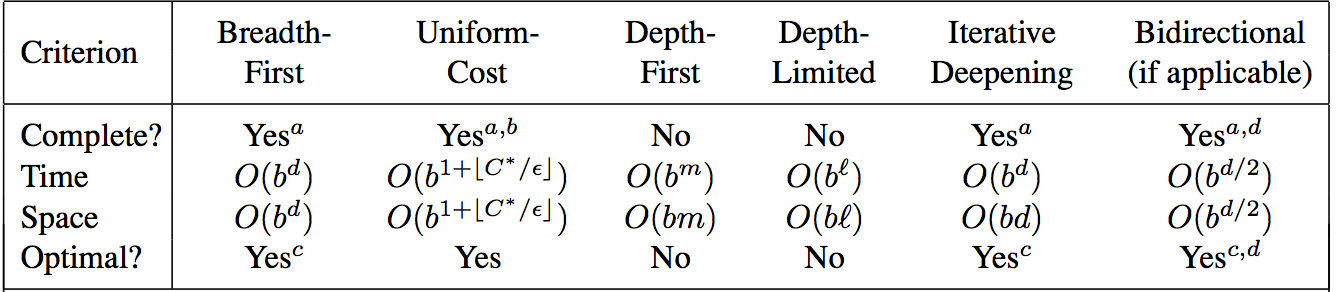
\includegraphics[width=\linewidth]{comparison.png}
  \caption{Comparison of uninformed search strategies. \(b\) is the branching 
  factor; \(d\) is the depth of the shallowest solution; \(m\) is the maximum depth 
  of the search tree; \(l\) is the depth limit. Superscript caveats are as follows:
  \(^a\) complete if \(b\) is finite; \(b\) complete if step costs \(\geq \epsilon\)
   for positive \(\epsilon\); \(^c\) optimal if step costs are all identical; 
  \(^d\) if both directions use breadth-first search.}
  \label{fig:comparison}
\end{figure}

\section{Informed Search Algorithms}
An informed search strategy is one that uses problem-specific knowledge beyond
the definition of the problem itself. The general approach considered is an
instance of a general graph or tree search in which a node is chosen for 
expansion based on its \textbf{evaluation function}, \(f(n)\). Most best-first
algorithms include as a component of \(f\) a \textbf{heuristic function},
denoted by \(h(n)\), which is an estimated cost of the cheapest path from
the state at node \(n\) to a goal state. We use the constraint that if \(n\)
is the goal node then \(h(n) = 0\).
\subsection{Greedy Best-First Search}
This algorithm uses \(f(n) = h(n)\). Due to its greedy nature it is not 
optimal and is also incomplete even in a finite state space, like DFS. The graph
version of this algorithm is complete in finite spaces, but not infinite ones.
The worse case space and time complexity for the tree version is \(O(b^m)\),
where \(m\) is the maximum depth of the search tree.
\subsection{A* Search}
This search evaluates nodes by using:
\begin{equation}
        f(n) = g(n) + h(n)
\end{equation}
Since \(g(n)\) gives the path cost from the start node to node \(n\), and 
\(h(n)\) is the estimated cost of the cheapest path from \(n\) to the goal,
\(f(n)\) is the estimated cost of the cheapest solution through \(n\). Provided 
\(h(n)\) satisfies certain conditions, it's both complete and optimal.
\subsubsection{Conditions for Optimality: Admissibility and Consistency}
The first condition we require is \(h(n)\) be an \textbf{admissible heuristic},
meaning it is one that \emph{never overestimates} the cost to reach the goal.
Thus we have that \(f(n)\) never overestimates the true cost of a solution along
the current path through \(n\). The second condition required is 
\textbf{consistency}, or \textbf{monotonicity} for applications of A* to graph
search. A heuristic \(h(n)\) is consistent if:
\begin{equation}
        h(n) \leq c(n,a,n') + h(n')
\end{equation}
Where \(n'\) is the successor of \(n\) generated by action \(a\). This is a form
of the general \textbf{triangle inequality}, which says that each side of a 
triangle can't be longer than the sum of the other two sides. Here the triangle
is formed by \(n, n'\) and the goal \(G_n\) closest to \(n\).
\subsubsection{Optimality of A*}
We know that \emph{the tree-search version of A* is optimal if \(h(n)\) is 
admissible, while the graph-search version is optimal if \(h(n)\) is consistent.}
First let us establish: \emph{if \(h(n)\) is consistent then the values of
\(f(n)\) along any path are non-decreasing.} Suppose \(n'\) is a successor of
\(n\); then \(g(n') = g(n) + c(n,a,n')\) thus we have:
\begin{equation}
        f(n') = g(n') + h(n') = g(n) + c(n,a,n') + h(n') \geq g(n) + h(n) = f(n)
\end{equation}
The next step would be to prove that \emph{whenever A* selects a node for expansion,
the optimal path to that node has been found.} The fact that \(f\) costs are
non-decreasing along any path allows us to draw \textbf{contours} in the state
space. If \(C^*\) is the cost of the optimal solution path, then:
\begin{itemize}
        \item A* first expands all nodes with \(f(n) < C^*\).
        \item A* might then expand some of the nodes right on the ``goal contour''
              (where \(f(n) = C^*)\) before selecting the goal node.
\end{itemize}
Completeness requires that there be only finitely many nodes wih cost less than
or equal to \(C^*\), a condition only met if all step costs exceed some finite
\(\epsilon\) and if \(b\) is finite. One final observation is A* is 
\textbf{optimally efficient} for any given consistent heuristic i.e. no other
optimal algorithm is guaranteed to expand fewer nodes than A* because any 
algorithm that doesn't expand all nodes with \(f(n) < C^*\) runs the risk of 
missing the optimal solution. The space complexity is \(O(b^d)\) and the 
time complexity is \(O(b^\Delta)\), with 
\(\Delta \equiv h^* - h\), where \(h^*\) is the actual cost of getting from 
the root to the goal; and this is the formula for \textbf{absolute error}.
For constant step costs we have \(O(b^{\epsilon d})\), with 
\(\epsilon \equiv (h^* - h)/h^*\) which is the \textbf{relative error}.
\subsection{Heuristic Functions}
There are a few good heuristics used for the 8-puzzle like the number of 
misplaced tiles and the \textbf{manhattan distance} which is the sum of 
horizontal and vertical distances. One way to characterize the quality of 
a heuristic is the \textbf{effective branching factor}, \(b^*\), which is 
conventionally defined as an average number of nodes revisited of the current
iteration \(N\) as compared to the previous iteration \(N - 1\). If the total
number of nodes generated by A* for a particular problem is \(N\), and the 
solution depth is \(d\), then \(b^*\) is the branching factor that a uniform
tree of depth \(d\) would have in order to contain \(N + 1\) nodes. Thus:
\begin{equation}
        N + 1 = 1 + b^* + (b^*)^2 + ... + (b^*)^d
\end{equation}
If \(\forall\) nodes \(n, h_2(n) \geq h_1(n) \implies h_2\) \textbf{dominates} \(h_1\).
\subsubsection{Relaxed Problems}
A problem with fewer restrictions on the actions is called a \textbf{relaxed 
problem}. The state-space graph of the relaxed problem is a \emph{supergraph}
of the original state space because the removal of restrictions creates added
edges in the graph. Because edges are added to the state-space, any optimal
solution in the original problem is also a solution in the relaxed problem,
but the relaxed problems may have better solutions. Hence, \emph{the cost of 
an optimal solution to a relaxed problem is an admissible heuristic for the
original problem.} Furthermore, because the derived heuristic is an exact cost
for the relaxed problem, it muse obey the triangle inequality and is therefore 
consistent. If the relaxed problem is hard to solve, then the values of the 
corresponding heuristic will be expensive to compute. Since a collection of 
admissible heuristics are obtained, we can use an appropriate heuristic
on each node individually using:
\begin{equation}
        h(n) = \max\{h_1(n), ... , h_m(n)\}
\end{equation}
\subsection{Local Search Algorithms}
These algorithms operate using a single \textbf{current node} and generally
move only to neighbors of that node and the paths followed aren't retained.
Thus they have the advantages:
\begin{itemize}
        \item They use very little memory - usually a constant amount
        \item They can often find reasonable solutions in large or infinite
                state spaces
\end{itemize}
\subsubsection{Hill-Climbing Search}
The algorithm is shown in figure \ref{fig:hill}. It is comparative to ``trying
to find the top of Mount Everest in a thick fog while suffering from amnesia''.
It is also called \textbf{greedy local search}. Hill-Climbing gets stuck in
\textbf{local maxima/minima, ridges} and \textbf{plateaux}.
\begin{figure}
  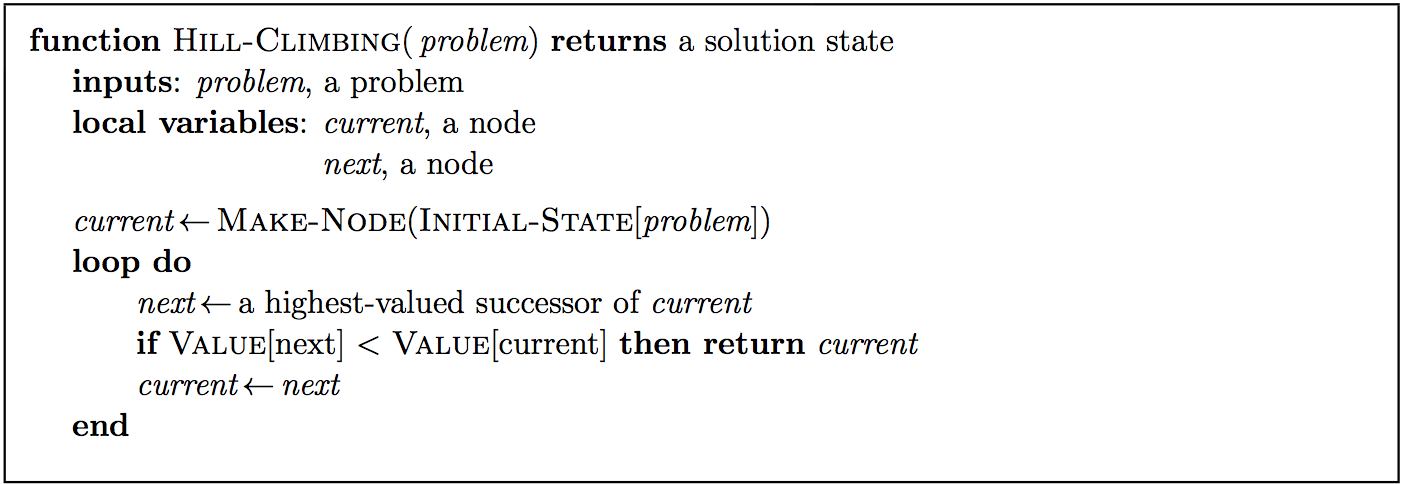
\includegraphics[width=\linewidth]{hill.png}
  \caption{Hill-Climbing Search.}
  \label{fig:hill}
\end{figure}
\section{Adversarial Search}
A \textbf{utility function} is defined as the final numeric value for a game
that ends in terminal state \(s\) for a player \(p\). A \textbf{zero-sum game}
is defined as one where the total payoff to every player is the same in 
every instance of the game.
\subsection{The Minimax Algorithm}
The algorithm is shown in figure \ref{fig:minimax}. The utility values of the 
leaf nodes are computed and the corresponding minimax values are backed up
the tree recursively. The time complexity of this algorithm is \(O(b^m)\), where
\(m\) is the maximum depth of the tree and there are \(b\) legal moves at each
point. The space complexity is \(O(bm)\) for an implementation that generates
all the actions at once and \(O(m)\) for an implementation that generates 
actions one at a time.
\begin{figure}
  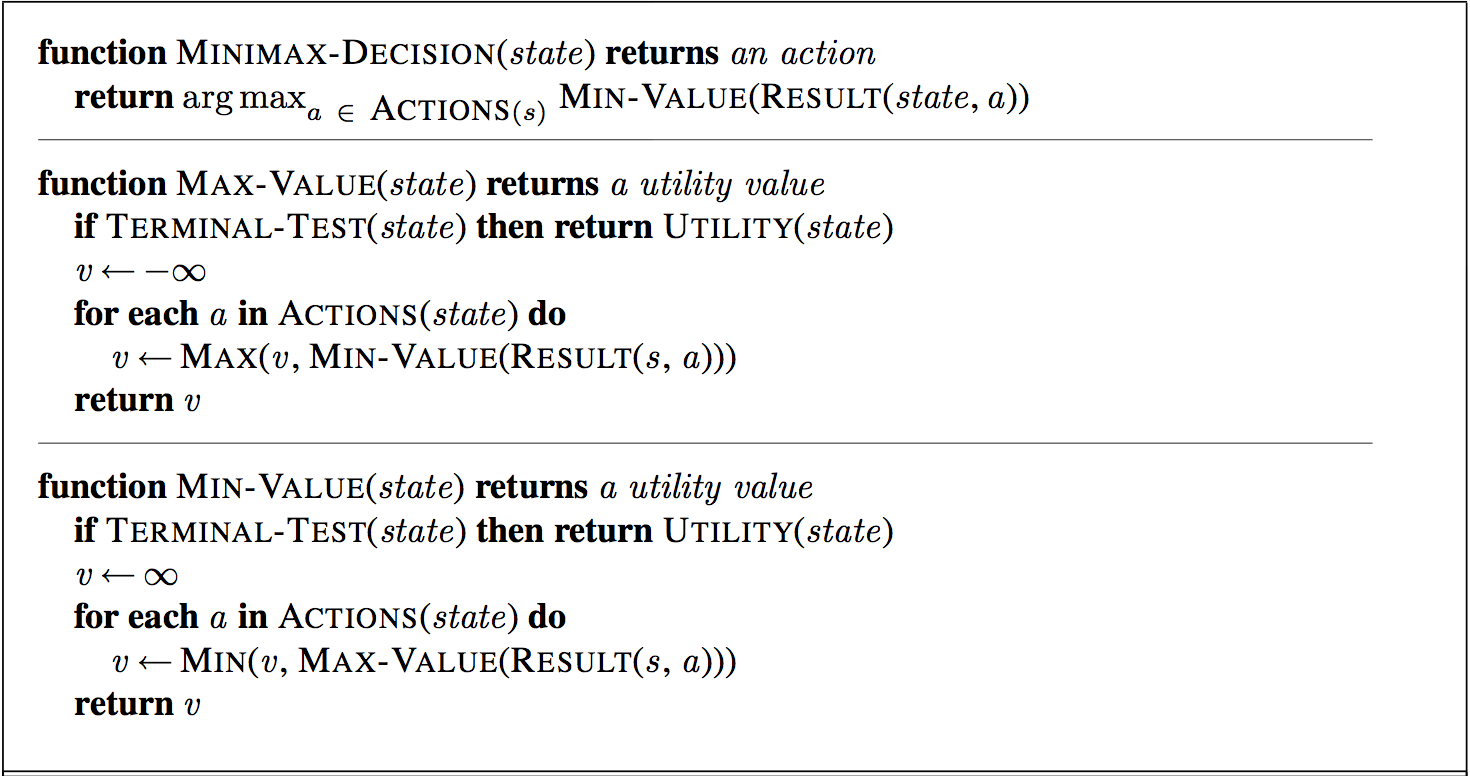
\includegraphics[width=\linewidth]{minimax.png}
  \caption{The Minimax Algorithm.}
  \label{fig:minimax}
\end{figure}
\subsection{Alpha-Beta Pruning}
A way to improve the abysmal complexity of Minimax is to use alpha-beta 
pruning, which prunes away branches that can't possibly influence the final
decision. \(\alpha\) is the best choice we have found so far for Max and 
\(\beta\) is the best choice for Min. The algorithm is applied in figure
\ref{fig:alpha-beta}. \textbf{Move ordering} can be applied to improve
complexity to \(O(b^{m/2})\) and the branching factor becomes \(\sqrt{b}\). If the 
successors are examined at random and not best-first the complexity increases
to \(O(b^{3m/4})\). The best moves in a game are called \textbf{killer moves}
and a killer move heuristic is used to find them. The hash table of 
previously seen moves is called a \textbf{transposition table}.
\begin{figure}
  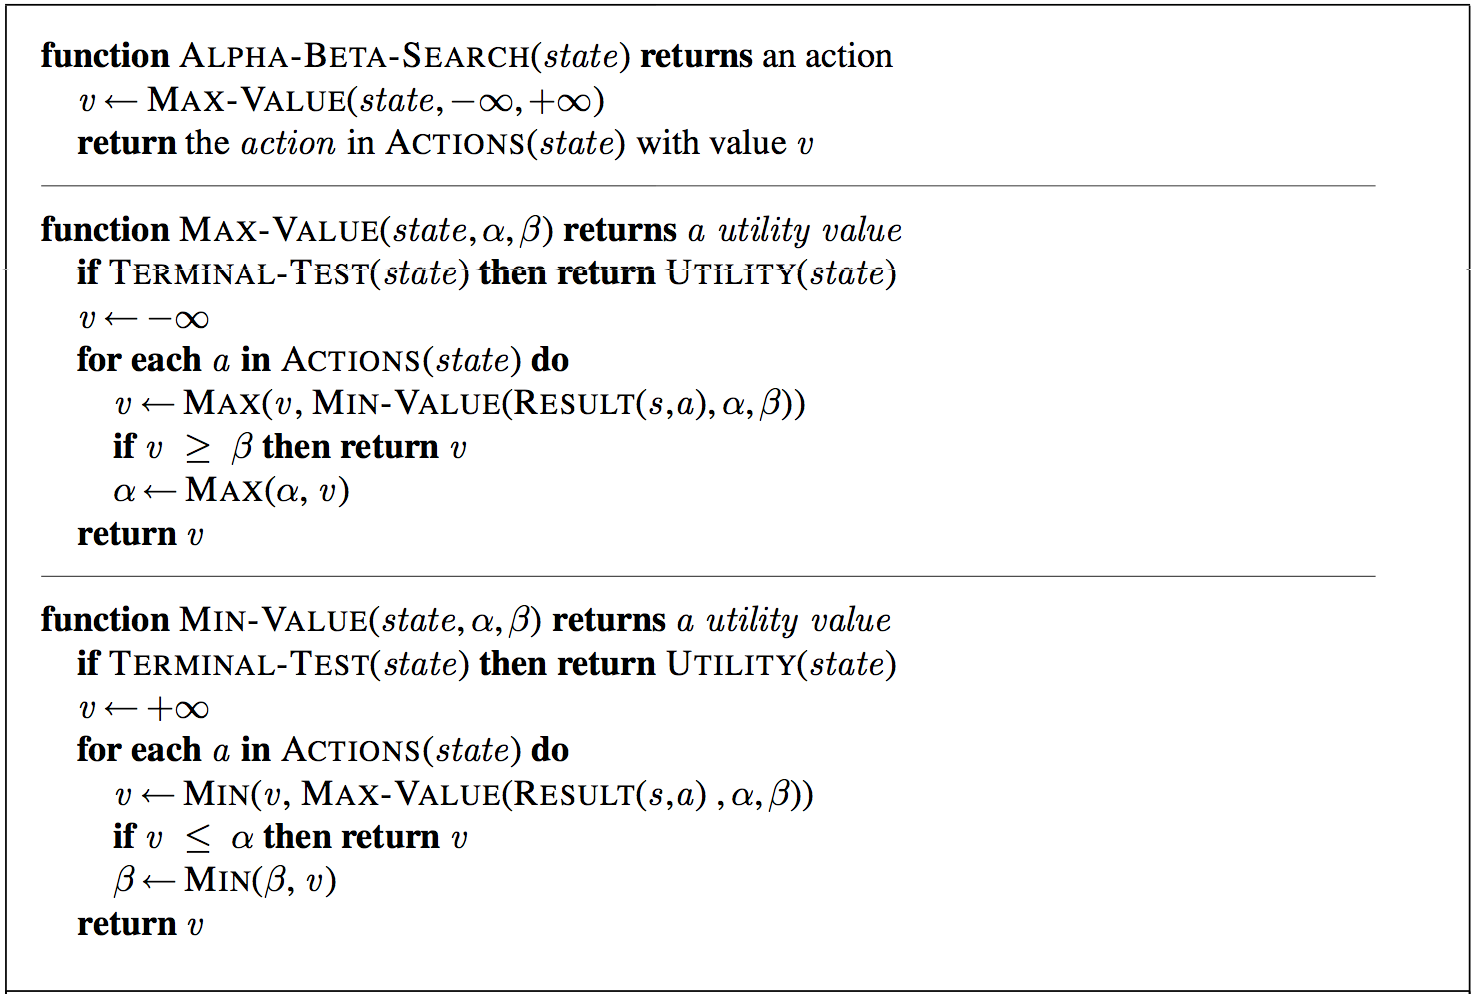
\includegraphics[width=\linewidth]{alpha-beta.png}
  \caption{Alpha-Beta Pruning.}
  \label{fig:alpha-beta}
\end{figure}
\subsection{Evaluation Functions}
An evaluation function returns an estimate of the expected utility from a given
position. This is useful as sometimes we want to stop our search at a depth 
limit and evaluate the leaf nodes using this function. Most evaluation
functions compute separate numerical contributions from each feature then
combine them to find the total value. These types of functions are also called
\textbf{weighted linear functions} because:
\begin{equation}
        E(s) = w_1f_1(s) + w_2f_2(s) + ... + w_nf_n(s) = \sum_{i=1}^{n} w_if_i(s)
\end{equation}
In \textbf{cutting off search} \texttt{isTerminal} and \texttt{utility} in minimax
are replaced by \texttt{cutoff} and \texttt{eval}. In stochastic games, 
chance nodes are added in addition to min/max nodes. The minimax values are also
replaced by \textbf{expected values}: the average over all possible outcomes of 
the chance nodes. This leads us to make \textbf{expecti-minimax} for games with
chance nodes.
\section{Machine Learning in Game Search}
We can automate the fine design choices in an evaluation function by using 
machine learning. We can use \textbf{book learning} to learn a sequence of
moves for important positions, like remembering what opening moves lead to 
what outcomes and remembering what moves led to a loss and avoiding them in
the future. \textbf{Search control learning} is used to learn how to make
search more efficient like order of move generation for \(\alpha-\beta\) and
learning a classifier to predict what depth we should search depending on the
current state. Weights in evaluation functions can also be learned to make
them agree with the true final utility.
\subsection{Gradient Descent Learning}
This is a a type of \emph{supervised learning} which is like the Hill-Climbing
algorithm, in that it starts at some point \(\mathbf w\) in the weight space and moves
to a neighboring lower point until we converge to the minimum possible loss.
The is hope that weights can be learned that closely approximate the true output.
Each weight is updated according to:
\begin{equation}
        w_i \leftarrow w_i - \alpha (z - t)f_i(s)
\end{equation}
\(\alpha\) is the \textbf{learning rate} which can be a constant or can decay
over time. The problems with this type of learning are:
\begin{itemize}
        \item Delayed reinforcement: reward maybe received after a few steps
        of applying the move
        \item Credit assignment: need to know which actions were responsible
        for the outcome
\end{itemize}
\subsection{Temporal Difference Learning}
Since supervised learning is for single-step prediction, TD is for multi-step
prediction. The correctness of the prediction is not known until a few steps
later, but intermediate steps can provide information about correctness. This
is a type of reinforcement learning. \textbf{TDLeaf}(\(\lambda\)) combines TD
and minimax to update evaluation function to reduce differences in rewards 
predicted at different levels of the search. The weight update rule applied is:
\begin{equation}
        w_j \leftarrow w_j + \alpha \sum_{i=1}^{N-1}\frac{\partial r(s_i^l, w)}{\partial w_j}\sum_{m=1}^{N-1}\lambda^{m-i}d_m
\end{equation}
Where \(r(s^l_i, w)\) is the reward for of a state (which is found at max cut-off
depth using minimax starting at \(s_i\)) using the weight \(w\). And \(d_i\) is
defined as difference between successive states:
\begin{equation}
        d_i = r(s^l_{i+1}, w) - r(r^l_i, w)
\end{equation}
\section{Constraint Satisfaction Problems}
We use a \textbf{factored representation} here for each state and when each 
value from the vector of variables of the states satisfies certain constraints,
we say a solution has been found. Problems such as this are called \textbf{constraint
satisfaction problems}. These problems are defined by:
\begin{itemize}
        \item \(X\) is a set of variables \(\{X_1, ... , X_n\}\).
        \item \(D\) is a set of domains \(\{D_1, ... , D_n\}\), one for each
        variable. Each \(D_i\) contains a set of allowable values,
        \(\{v_i,...,v_n\}\) for \(X_i\).
        \item \(C\) a set of constraints that specify allowable combination of
        values. Each \(C_i\) consists of a pair \(\langle scope, rel\rangle\)
        where \(scope\) is a tuple of variables that participate in the 
        constraint and \(rel\) is a relation that defines the values that 
        those variables can take on.
\end{itemize}
A CSP is solved by \textbf{assignment} of variables and if no constraints are 
violated, the assignment is \textbf{consistent}, if it assigns a value to each
variable then it is \textbf{complete} and \textbf{partial} otherwise. Solving
problems this way is useful as it eliminates large areas from the state space.
Domains can range from \textbf{continuous} to \textbf{discrete} and from
\textbf{finite} to \textbf{infinite}. Continuous domain problems can be 
solved using \textbf{linear programming}. A \textbf{unary constraint} restricts 
the value of one variable and a \textbf{binary} one restricts two variables. A
binary CSP (one with only binary constraints) can be represented by a constraint
graph. Confusingly, a constraint which involves an arbitrary number of variables
is called a \textbf{global constraint}. An example is \(Alldiff\) which says
that every variable involved in the constraint must have a different value. \\

\textbf{Cryptarithmetic} puzzles, which are essentially arithmetic operations
on number represented in their alphabetic form, can also be solved using CSPs.
A \textbf{constraint hypergraph} can be used to represent \(n\)-ary constraints,
using hypernodes (drawn as squares). Every finite-domain constraint can be 
reduced to a set of binary constraints if enough auxiliary variables are 
introduced. Another way to convert is the \textbf{dual graph} transformation:
create a new graph in which there will be one variable for each constraint in 
the original graph, and one binary constraint for each pair of constraints in
the original graph that share variables. Global constraint are preferred because
they are less error-prone and allow us to design special-purpose inference 
algorithms not available for a set of more primitive constraints. There are
also \textbf{preference constraints} indicating which solutions are preferred,
which can be realized by penalizing lesser-preferred solutions; such problems
are called \textbf{constraint optimization problems}.
\subsection{Constraint Propagation}
In regular state space an algorithm can only search, but with CSPs, in addition
to search, we can do an inference called \textbf{constraint propagation}: using
constraints to reduce the number of legal values for a variable, which in turn 
can reduce the legal values for another variable.
\subsubsection{Node Consistency}
A single variable (a node in the CSP network) is node-consistent if all the 
values in the variable's domain satisfy the variable's unary constraints. A 
network can be node-consistent if every variable in the network in node-consistent.
\subsubsection{Arc Consistency}
A variable is arc-consistent if every value in its domain satisfies the 
variable's binary constraint i.e. \(X_i\) is arc-consistent with respect to 
another variable \(X_j\) if:
\begin{equation}
        \forall v_i \in D_i, \exists v_j \in D_j \text{ s.t. } \text{the binary constraint } (X_i, X_j) \text{ is satisfied}
\end{equation}
A network is arc-consistent if every variable is arc-consistent with every
other variable. The arc-consistency algorithm is shown in figure \ref{fig:ac3}.
The time complexity of AC-3 is \(O(cd^3)\), where \(c\) are the binary 
constraints (arcs), \(d\) is the the maximum domain size of one of \(n\) 
variables and also note that checking consistency of an arc can be done in 
\(O(d^2)\) time.
\begin{figure}
  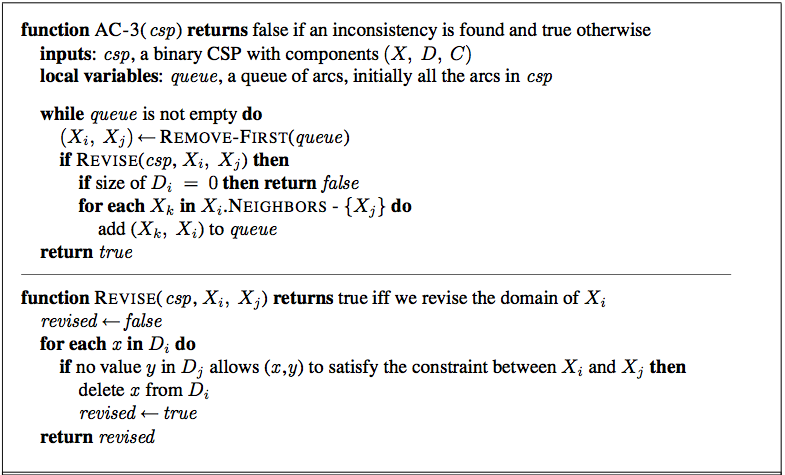
\includegraphics[width=\linewidth]{ac3.png}
  \caption{The Arc-Consistency Algorithm AC-3.}
  \label{fig:ac3}
\end{figure}
\subsection{Backtracking Search}
A problem is \textbf{commutative} if the order of application of any given
set of actions has no effect on the outcome. We use \textbf{backtracking search}
for a depth-first search that chooses values for one variable at a time and
backtracks when a variable has no legal values left to assign. The algorithm is
shown in figure \ref{fig:backtrack}. The complexity of this algorithm is 
\(O(d^n)\) where \(n\) is the number of variables.
\begin{figure}
  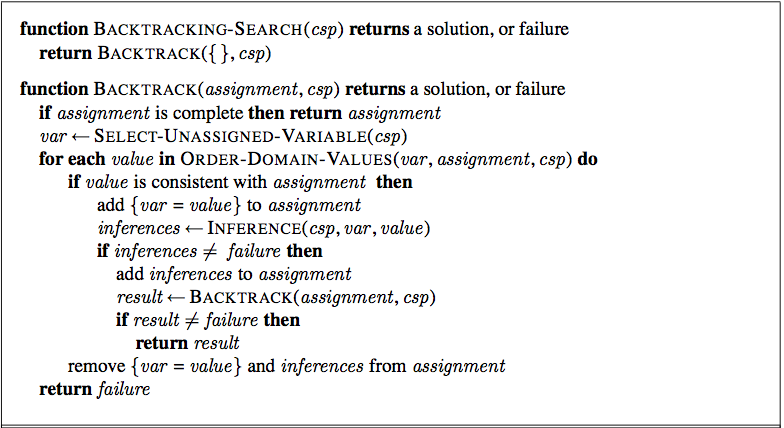
\includegraphics[width=\linewidth]{backtrack.png}
  \caption{Backtracking search algorithm.}
  \label{fig:backtrack}
\end{figure}
The algorithm can be improved by thinking about questions like:
\begin{itemize}
        \item Which variable should be assigned next and what order should
        its values be tried?
        \item What inferences should be performed at each step in the search?
        \item When the search arrives at an assignment that violates a 
        constraint, can the search avoid repeating this failure?
\end{itemize}
When we choose an unassigned variable in the CSP, we can choose the most 
constrained one thereby reducing the size of the search tree, doing so is called
the \textbf{minimum-remaining-values} heuristic. Another technique used is the 
\textbf{degree heuristic} which chooses the variable involved in the largest
 number of constraints. Once a variable has been selected, the algorithm must
 choose which of its values to examine first, the \textbf{least-constraining-value}
 heuristic can be used for this. Doing this would leave maximum flexibility 
 for subsequent variable assignments. One of the simplest form of inference
 is called \textbf{forward checking}; whenever a value is chosen for \(X\),
 the forward checking process establishes arc consistency for it.\\

 \textbf{Maintaining Arc Consistency}, MAC, is used to maintain arc consistency
 throughout the graph. So after variable \(X_i\) is assigned a value, 
 \texttt{inference} calls AC-3 but only starting with arcs \((X_j, X_i)\) for
 all \(X_j\) that are unassigned variables that are neighbors of \(X_i\).
 \subsection{The Structure of Problems}
 \textbf{Independent subproblems} are ones which combine to yield the final
 solution to the problem. Independence can be ascertained by finding the
 \textbf{connected components} of a constraint graph, each problem corresponds
 to a subproblem \(CSP_i\). If assignment \(S_i\) is a solution of \(CSP_i\),
 then \(\bigcup _iS_i\) is a solution of \(\bigcup _iCSP_i\). Solving problems
 in this way reduces the complexity from \(O(d^n)\) to \(O(d^cn/c)\). A 
 constraint graph is a tree if any two variables are connected by only one
 path and \emph{any tree-structured CSP can be solved in linear time with
 respect in the number of variables}. The key is \textbf{directed arc consistency}:
every \(X_i\) is arc-consistent with each \(X_j\) for \(j > i\) if and only if
a CSP is defined to be DAC under any ordering of variables \(X_i, X_2,...,X_n\).\\

\begin{figure}
  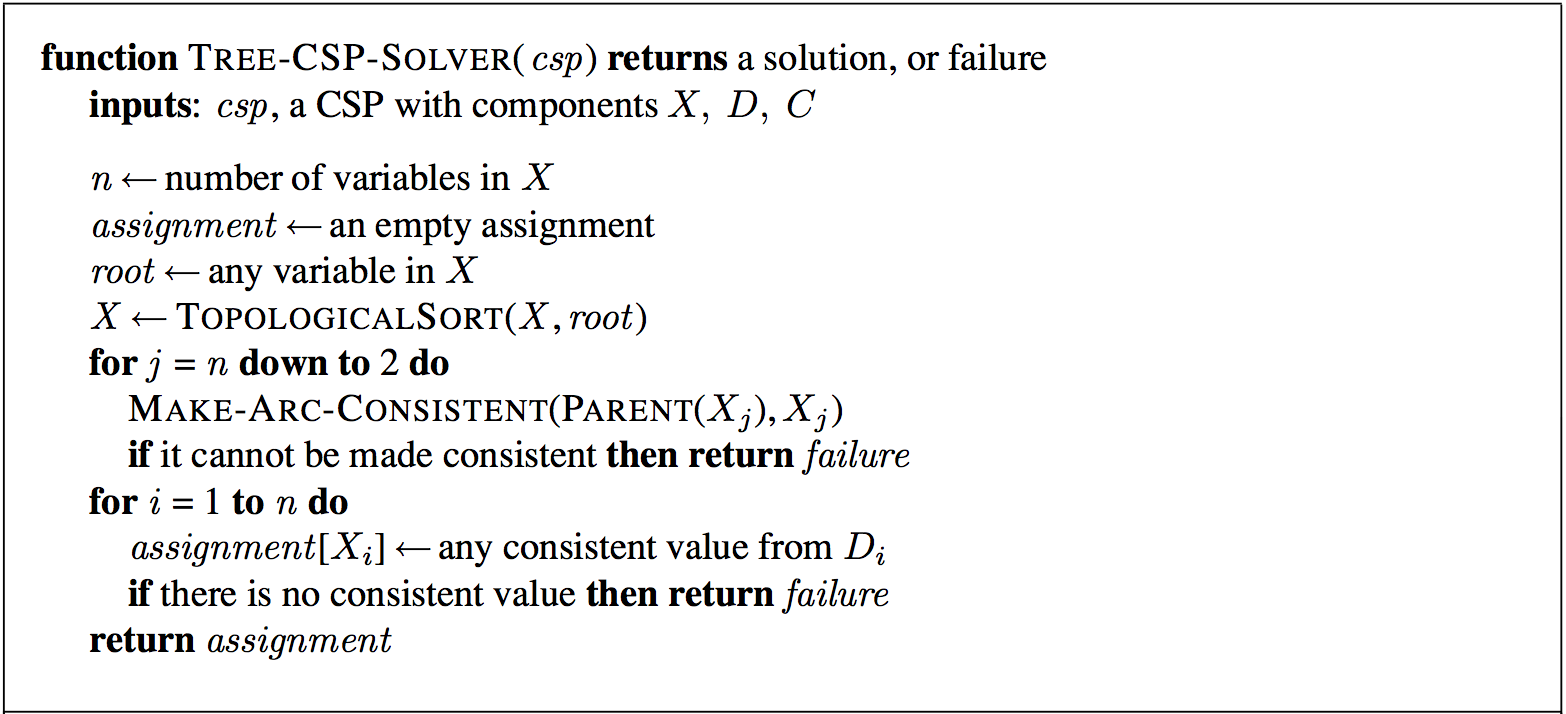
\includegraphics[width=\linewidth]{tcs.png}
  \caption{The Tree CSP Solver algorithm.}
  \label{fig:tcs}
\end{figure}
An ordering of variables such that each variable appears after its parent in
the tree is called \textbf{topologically sorted}. The tree-CSP-solver is given
in figure \ref{fig:tcs}. Now that we have an efficient algorithm for trees, we 
can think of converting graphs to trees: by either removing nodes or by 
collapsing nodes together. If a value for a node is set it can considered as 
not being there at all. The general algorithm is:
\begin{itemize}
        \item Choose a subset \(S\) of the CSP's variables such that the 
        constraint graph becomes a tree after removal of \(S\) which is called
        the \textbf{cycle cutset}
        \item For each possible assignment to the variables in \(S\) that satisfy
        all the constraints in \(S\),
        \begin{itemize}
                \item remove from the domains of the remaining variables any
                values that are inconsistent with the assignment for \(S\)
                \item if the remaining CSP is a solution, then return it with 
                the assignment to \(S\)
        \end{itemize}
\end{itemize}
If the cycle cutset size is \(c\) then time complexity is \(O(d^c\cdot (n-c)d^2)\);
we have to try each of the \(d^c\) combinations of values for the variables in
\(S\), and for each combination we must solve a tree problem of size \(n-c\).
Finding the \emph{smallest} cycle cutset is NP-hard, but efficient algorithms 
like \textbf{cutset conditioning} can be used, which instantiates, in all ways,
a set of variables such that the remaining constraint graph is a tree.
\section{Quantifying Uncertainty}
The problems with keeping track of a belief state - a representation of the set
of all possible world states that it might be in - are:
\begin{itemize}
        \item The agent must consider every logical possible explanation for
        the observations, no matter how unlikely, leading to impossibly large
        and complex belief-state representations.
        \item A correct contingent plan that handles every eventuality can 
        grow arbitrarily large and must consider arbitrarily unlikely 
        contingencies.
        \item Sometimes there is no plan that is guaranteed to achieve the 
        goal. It must have some way to compare the merits of plans that are 
        not guaranteed.
\end{itemize}
Decision theory essentially states that an agent is rational if and only if it 
chooses the action that yields the highest expected utility, averaged over all
the possible outcomes of the action. The basic axioms of probability theory say
that every possible world has a probability between 0 and 1 and that the total
probability of the set of possible worlds is 1:
\begin{equation}
        0 \leq P(\omega) \leq 1 \text{ for every } \omega \text{ and } \sum_{\omega \in \Omega} P(\omega) = 1
\end{equation}
Conditional probabilities are defined by:
\begin{equation}
        P(a|b) = \frac{P(a \land b)}{P(b)}
\end{equation}
Note also the inclusion-exclusion principle:
\begin{equation}
        P(a \lor b) = P(a) + P(b) - P(a \land b)
\end{equation}
The following equations give marginal probability and conditioning respectively:
\begin{equation}
        \mathbf{P(Y) = \sum_{z \in Z} P(Y, z)}
        \mathbf{P(Y) = \sum_{z \in Z}P(Y|z)}P(\mathbf{z})
\end{equation}
Let \(\mathbf{E}\) be the list of evidence variables, let \(\mathbf{e}\) be 
the list of observed values for them and let \(\mathbf{Y}\) be the remaining
unobserved variables and then we have:
\begin{equation}
        \mathbf P(X|\mathbf e) = \alpha \mathbf P(X, \mathbf e) = \alpha \sum_\mathbf y \mathbf P(X, \mathbf e, \mathbf y)
\end{equation}
Independence can be written as:
\begin{equation}
        P(a|b) = P(a) \text{ or } P(a \land b) = P(a)P(b)
\end{equation}
And independence for random variables can be written as:
\begin{equation}
        \mathbf P(X|Y) = \mathbf P(X) \text{ or } \mathbf P(X, Y) = \mathbf P(X) \mathbf P(Y)
\end{equation}
\subsection{Bayes' Rule}
The \textbf{Bayes' rule} is given as:
\begin{equation}
        P(b \mid a) = \frac{P(a \mid b)P(b)}{P(a)}
\end{equation}
The Bayes' rule for multivariate variables is:
\begin{equation}
        \mathbf P(Y \mid X) = \frac{\mathbf P(X \mid Y) \mathbf P(Y)}{\mathbf P(X)}
\end{equation}
Gives \(\alpha\) is is the normalization constant needed to make entries in 
\(\mathbf P(Y|X)\) sum to 1, the Bayes' rule becomes:
\begin{equation}
        \mathbf P(Y|X) = \alpha \mathbf P(X|Y) \mathbf P(Y)
\end{equation}
The \textbf{conditional independence} of two variables \(X\) and \(Y\), given 
a third variable \(Z\) is:
\begin{equation}
        \mathbf P(X,Y|Z) = \mathbf P(X|Z) \mathbf P(Y|Z)
\end{equation}
The following equation illustrates how a single cause directly influences a 
number of effects, all of which are conditionally 
independent, given the cause:
\begin{equation}
        \mathbf P(Cause, Effect_1,...,Effect_n) = \mathbf P(Cause) \prod _i \mathbf P(Effect_i|Cause)
\end{equation}
Such a probability distribution function is called a \textbf{naive Bayes} 
model as it is often used in cases where the ``effect'' variables are not 
actually conditionally independent given the cause variables.
\section{Bayesian Networks}
A Bayesian network is a directed graph in which each node is annotated with 
quantitative probability information and has the following features:
\begin{itemize}
        \item Each node corresponds to a random variable, which may be discrete 
        or continuous.
        \item A set of directed links or arrows connects pairs of nodes. If 
        there is an from from node \(X\) to node \(Y\), \(X\) is the parent of 
        \(Y\). The graph has no directed cycles and is therefore a DAG.
        \item Each node \(X_i\) has a conditional probability distribution \(\mathbf P(X_i|Parents(X_i))\)
        that quantifies the effect of the parents on the node.
\end{itemize}
A \textbf{conditional probability table} for boolean \(X_i\) with \(k\) boolean 
parents has \(2^k\) rows for the combination of parent values. If each variable
has no more than \(k\) parents, the complete network requires \(O(n\cdot 2^k)\)
numbers as compared to \(O(2^n)\) for the full joint distribution.
\subsection{Representing Bayesian Networks}
A generic entry in the joint distribution is the probability of a conjunction of
particular assignments to each variable, such as \(P(X_1=x_1 \land ... \land X_n = x_n)\)
which we abbreviate to \(P(x_1,...,x_n)\) and is given by:
\begin{equation}
        P(x_1,...,x_n) = \prod_{i=1}^n P(x_i|parents(X_i))
\end{equation}
The chain rule is useful when constructing Bayesian networks:
\begin{equation}
        P(x_1,...,x_n) = \prod_{i=1}^n P(x_i|x_{i-1},...,x_1)
\end{equation}
Also note that for every variable \(X_i\) in the network:
\begin{equation}
        \mathbf P(X_i|X_{i-1},...,X_i) = \mathbf P(X_i|Parents(X_i))
\end{equation}
Provided that \(Parents(X_i) \subseteq \{X_{i-1},...,X_1\}\). What this equation 
says is that the Bayesian network is a correct representation of the domain only 
if each node is conditionally independent of its other predecessors in the node 
ordering, given its parents, which can be satisfied if:
\begin{itemize}
        \item Node: First determine the set of variables required to model the 
        domain and order them. Any order will work, but the network will be more 
        compact if the order is such that causes precede effects.
        \item Links: For \(i=1\) to \(n\) do:
                \begin{itemize}
                        \item Choose from \(X_1,...,X_{i-1}\) a minimal set of 
                        parents for \(X_i\) such that the previous equation is 
                        satisfied
                        \item For each parent insert a link from parent to \(X_i\)
                        \item Write down the CPT, \(\mathbf P(X_i|Parents(X_i))\)
                \end{itemize}
\end{itemize}
\subsection{Exact Inference in Bayesian Networks}
The basic task for any probabilistic inference systems is to compute the 
posterior probability distribution for a set of \textbf{query variables}, given 
some observed \textbf{event} i.e. some assignment of values to a set of 
\textbf{evidence variables}. A complete set of variables is \(\mathbf X=\{X\} \cup \mathbf E \cup \mathbf Y\).
Where \(\mathbf Y\) are the hidden variables and \(\mathbf E\) denotes evidence 
variables. We can infer by enumeration:
\begin{equation}
        \mathbf P(X|\mathbf e) = \alpha \mathbf P(X,\mathbf e) = \alpha \sum_{\mathbf y} \mathbf P(X,\mathbf e,\mathbf y)
\end{equation}
But this is computationally expensive as a recursive DFS would give us \(O(n)\)
space complexity and \(O(d^n)\) time complexity. We can use \textbf{variable
elimination} here to remember past computations. Note that we use \textbf{pointwise
product} here which is described by:
\begin{equation}
        \mathbf f(X_1...X_j,Y_1...Y_k,Z_1...Z_l)=\mathbf f_1(X_1...X_j,Y_1...Y_k)\times \mathbf f_2(Y_1...Y_k,Z_1...Z_l)
\end{equation}
\section{Making Complex Decisions}
Here we look at complex application that can involve multi-agent systems, where 
multiple agents are competing for a scarce resource.
\subsection{Mechanism Design}
Here we would like to design a game whose solutions, consisting of each agent 
pursuing its own rational strategy, result in the maximization of some global 
utility function. This problem is called \textbf{mechanism design} or \textbf{
inverse game theory}. Formally a mechanism consists of:
\begin{itemize}
        \item A language for describing the set of allowable strategies that 
        agents may adopt.
        \item A distinguished agent, called the \textbf{center}, that collects 
        reports of strategy choices from the agents in the game.
        \item An outcome rule, known to all agents, that the center uses to 
        determine payoffs to each agent, given their strategy choices.
\end{itemize}
\subsection{Auctions}
Each bidder \(i\) has a utility value \(v_i\) for having the item. Given \(v_i\),
each bidder get a chance, at the appropriate time or times in the auction, to 
make a bid \(b_i\). The highest bid, \(b_{max}\) wins the item, but the price 
paid need not be \(b_{max}\); that's part of the mechanism design.\\

The best-known mechanism is the \textbf{ascending bid} or an \textbf{English 
auction}, in which the center start by asking for a minimum bid \(b_{min}\). If
some bidder is willing to pay that amount, the center then asks for \(b_{min}+d\).
An auction is \textbf{efficient} if the goods go to the agent who values them 
most. The most important things an auction design can do is to encourage a 
sufficient number of bidders to enter the game and discourage them from engaging
in \textbf{collusion}, which is an unfair or illegal agreement by two or more 
bidders to manipulate prices. It is desirable that the bidders have a \textbf{
dominant strategy}, meaning a strategy that works against all other strategies,
and therefore can be adopted without regard for other agents' strategies. A 
mechanism where agents have this strategy is called a \textbf{strategy-proof} 
mechanism. And if the strategy involves revealing their true value, \(v_i\), then
it is called a \textbf{truth-revealing} auction. A disadvantage of the ascending
bid auction is that it can discourage competition and another disadvantage is 
that it has high communication costs.\\

A \textbf{Dutch auction} is typically, open-cry and descending auction. Here the
auctioneer starts by asking for an extremely high initial price and repeatedly 
lowers the price of the good in small steps. The auctions ends when someone 
makes a bid at the current offer price. The price paid by the winner is the 
price when their bid was made. They can suffer from similar problems as English
auctions. \\

An alternative mechanism is the \textbf{sealed-bid auction} where each bidder 
makes a single bid and communicates it only to the auctioneer. Here the agent 
would have to do some computation as to what the other bids could be. In the 
\textbf{sealed-bid second-price auction} or a \textbf{Vickrey auction}, the 
winner pays the price of the second-highest bid, \(b_o\), rather than paying his
own bid. This causes the agent to not deliberate on other agents' decisions, but 
just bid \(v_i\), thus the mechanism is truth-revealing. Note that the utility 
of agent \(i\) in terms of his bid \(b_i\), his value \(v_i\), and the best bid
among other agents \(b_o\) is:
\begin{equation}
        u_i = 
        \begin{cases}
                (v_i - b_o) & \text{if } b_i > b_o \\
                0 & \text{otherwise} \\
        \end{cases}
\end{equation}
Note that the expected value to the seller is \(b_o\), which is the same expected
return as the limit of the English auction as the increment \(d\) goes to zero.
The \textbf{revenue equivalence theorem} states that, with a few minor caveats,
any auction mechanism where risk-neutral bidder have values \(v_i\) known to 
themselves (but know a probability distribution from which those values are 
sampled), will yield the same expected revenue. This means that the various 
mechanisms aren't competing on the basis of revenue generation, but rather on
other qualities.
\section{Robotics}
Robots are physical agents that perform tasks by manipulating the physical world.
To do so, they are equipped with \textbf{effectors} and \textbf{sensors}. There 
are three major types of robots:
\begin{itemize}
        \item \textbf{Manipulators}: or robot arms, are physically anchored to 
        their workplace.
        \item \textbf{Mobile robots}: which move about their environment using
        wheels, legs, etc. Examples are UGVs, UAVs, AUVs, etc.
        \item \textbf{Mobile manipulator}: which combines mobility with manipulation.
        They can apply their effectors further afield than anchored manipulators
        can, but their task is made harder because they don't have the rigidity
        that the anchor provides.
\end{itemize}
Effectors can be talked about using the concept of \textbf{degrees of freedom},
an AUV would have 6 DOFs: \((x,y,z)\) and angular rotation i.e. \(yaw,roll,pitch\).
These six degrees define the \textbf{kinematic state} or \textbf{pose} of the robot.
A robot is \textbf{nonholonomic} if it has more effective DOFs than controllable
DOFs and \textbf{holonomic} if the two numbers are the same. There are many 
sources of uncertainty in motion actions like slippage, inaccurate joint 
encoding, rough surfaces, obstacles, effector breakdown (injuries), etc. There
are different types of sensors: range finders like sonar, laser range finder, 
radar, GPS; imaging sensors like visual and infrared cameras; proprioceptive 
sensors like shaft decoders (joint, wheels), inertial sensors, force sensors,
torque sensors, etc. Therefore the agent must make assumptions on how the world 
works.
\subsection{Localization}
Figure \ref{fig:localization} shows an action, \(A_t\) at time \(t\) in state 
\(X_{t+1}\) and observation \(Z_{t+1}\). We can use particle filtering to 
produce approximate position estimates. First we start with random samples from
uniform prior distribution for the robot position and then update the likelihood
of each sample using sensor measurements. Finally, we re-sample according to 
updated likelihoods. We need to continuously update our distribution for the 
current state using the latest measurements. The uncertainty of the robot's 
state grows as it moves until we find a landmark. We assume that landmarks are 
identifiable.
\begin{figure}
  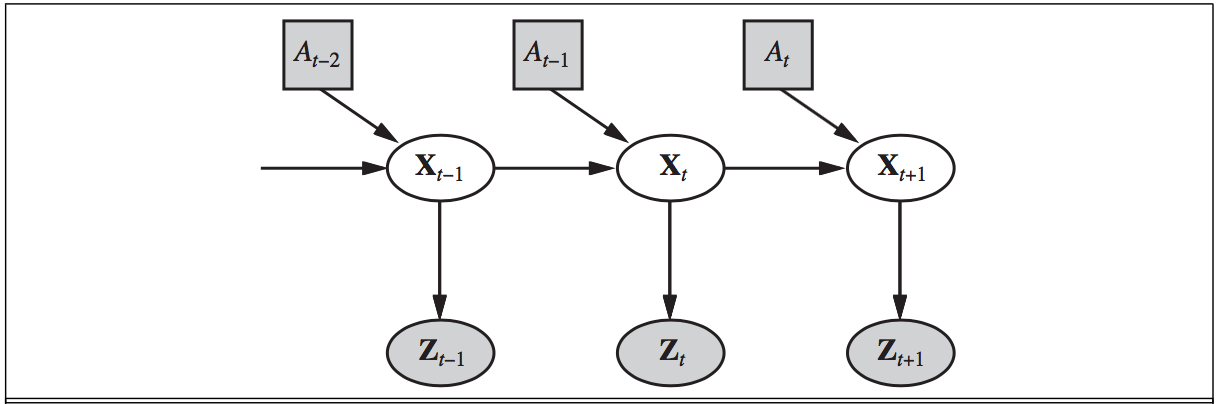
\includegraphics[width=\linewidth]{localization.png}
  \caption{An example robot perception.}
  \label{fig:localization}
\end{figure}
Localization is essentially: given map and observed landmarks, update pose 
distribution and \textbf{mapping} is: given pose and observed landmarks, update
map distribution. Consequently, \textbf{Simultaneous Localization and Mapping} 
or SLAM is given observed landmarks, update pose and pose distribution. In the
probabilistic formulation of SLAM, the landmark locations \(L_1,...,L_k\) are 
added to the state vector and we proceed as for localization. Given the current 
probability distribution, \(P(H)\) and the new measurement \(M\), the update 
probability distribution is:
\begin{equation}
        P(H) \gets \frac{P(M|H)}{P(M)}P(H)
\end{equation}
This is sometimes called the Bayesian update rule.
\subsection{Motion Planning}
We now have to plan in the \textbf{configuration space} defined by the robot's DOFs. The 
problem is that there \(\infty^d\) states and we need to convert them into 
finite states. This can be done by:
\begin{itemize}
        \item \textbf{Cell decomposition}: divide up space into simple cells, 
        each of which can be traversed easily. The problem here is that there
        maybe no path in pure free space cells which is solved by recursive 
        decomposition of free and obstacle, mixed, cells.
        \item \textbf{Skeletonization}: identify finite number of easily connect 
        points/lines that form a graph such that ny two points are connected by 
        a path on the graph. Figure \ref{fig:maps} shows voronoi diagram in 
        which the locus of points are equidistant from obstacles, but this 
        doesn't scale well to higher dimensions. It also shows a probabilistic 
        roadmap, but the problem is that we may need to generate enough points 
        to ensure that every start/goal pair is connected through the graph.
\end{itemize}
\begin{figure}
  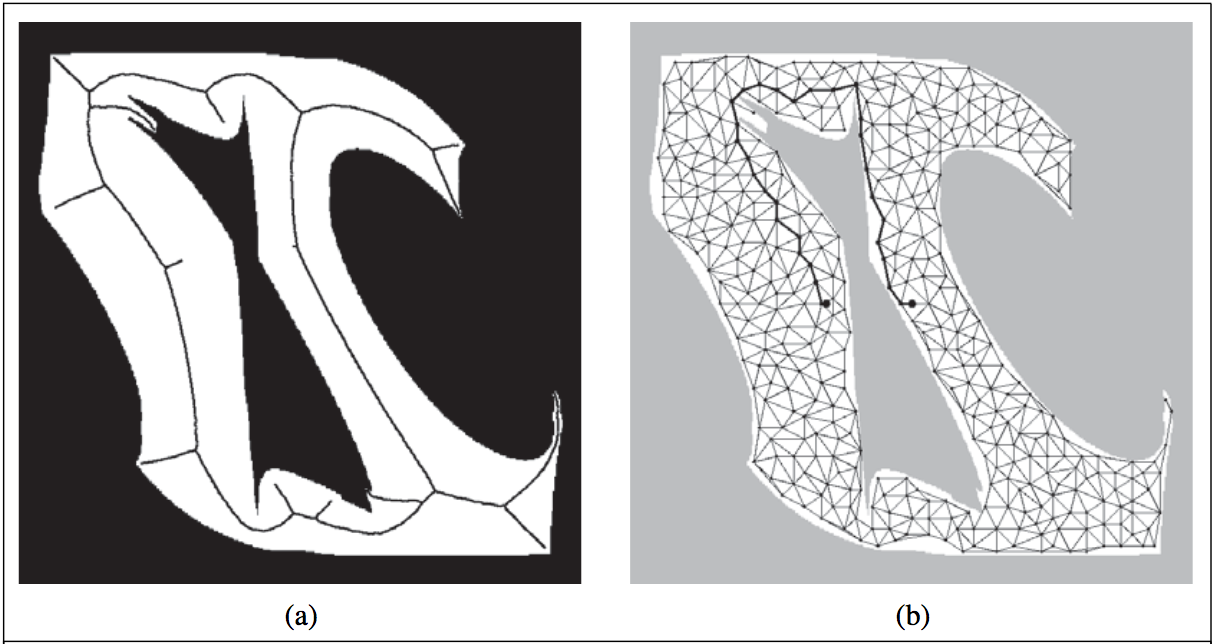
\includegraphics[width=\linewidth]{maps.png}
  \caption{(a) shows a voronoi map and (b) shows a probabilistic roadmap.}
  \label{fig:maps}
\end{figure}
\end{document}